\documentclass[conference]{IEEEtran}
\usepackage[T1]{fontenc}
\usepackage{graphicx}
\usepackage{amsmath}
\usepackage{booktabs}
\usepackage{tikz}
\usetikzlibrary{positioning, arrows.meta}
\usepackage{url}

\begin{document}

\title{Quantum vs. Classical Approaches for Streaming Data Analytics: An Experimental Study on Drift-Adaptive Quantum Machine Learning}

\author{%
\IEEEauthorblockN{Sumit Hulke}
\IEEEauthorblockA{Roll No. 2023BCS0026 \\
% TODO: insert institution name
Department of Computer Science and Engineering}
\and
\IEEEauthorblockN{Adnan Omar}
\IEEEauthorblockA{Roll No. 2023BCS0035 \\
Department of Computer Science and Engineering}
\and
\IEEEauthorblockN{Ashwin S}
\IEEEauthorblockA{Roll No. 2023BCS0044 \\
Department of Computer Science and Engineering}
\and
\IEEEauthorblockN{Mubaris}
\IEEEauthorblockA{Roll No. 2023BCS0062 \\
Department of Computer Science and Engineering}
}

\maketitle

\begin{abstract}
Quantum machine learning (QML) is increasingly proposed as an alternative to classical
streaming ML, yet published evaluations are batch-oriented and say little about behaviour
under concept drift and per-event latency budgets. We present \textsc{Qompare}, an
end-to-end streaming analytics pipeline that evaluates an eight-model matrix --- classical
and quantum model families, each in static and drift-adaptive variants --- with strict
prequential (test-then-train) evaluation on the non-stationary ELEC2 electricity market
stream (45{,}312 half-hourly events), with real data flowing through Apache Kafka, an
online feature worker, InfluxDB, and Grafana. We reproduce the Hoeffding-tree baseline of
Domingos and Hulten, adapt a variational quantum classifier and a fidelity quantum kernel
classifier from the recent QML literature, and contribute a dual drift-adaptation
mechanism: ADWIN-triggered warm-started SPSA fine-tuning for variational models and
sliding support-set refresh for kernel models, against a capacity-matched classical RBF
control. Across 189 detected drift events, adaptation improves quantum accuracy by
4--5 percentage points over frozen models. However, the adaptive quantum kernel (64.2\%)
only matches the classical RBF kernel (64.4\%) at roughly $20\times$ the per-event
simulation latency, and both trail an adaptive Hoeffding tree (80.8\%). On this task, the
quantum advantage does not survive streaming constraints.
\end{abstract}

\begin{IEEEkeywords}
streaming data analytics, quantum machine learning, concept drift, prequential evaluation,
variational quantum classifiers, quantum kernels, Hoeffding trees
\end{IEEEkeywords}

\section{Introduction}
\label{sec:intro}

Streaming analytics systems must classify high-velocity event data under strict time and
memory budgets while the underlying process keeps changing. Classical streaming machine
learning answers this with incremental models --- most famously the Hoeffding tree of
Domingos and Hulten~\cite{domingos2000} --- and with drift detectors such as
ADWIN~\cite{bifet2007adwin}. Quantum machine learning (QML) promises complementary
benefits: exponentially large feature spaces, compact parametrisation, and claimed sample-efficiency gains in kernel and variational
settings~\cite{schuld2019,herbst2024,tscharke2023}. Almost all published QML results,
however, are obtained \emph{offline}, on shuffled batch data, under no latency budget and
no distribution shift. Whether any quantum advantage survives a true streaming
environment is untested.

This paper closes that gap with three contributions:
\begin{enumerate}
  \item \textbf{A reproduction and adaptation set:} the Hoeffding tree (VFDT) of~\cite{domingos2000}
    is reproduced as the classical baseline; the variational-quantum and quantum-kernel
    models of~\cite{herbst2024} and~\cite{tscharke2023} are adapted to streaming binary
    classification on the ELEC2 benchmark.
  \item \textbf{A drift-adaptive QML mechanism:} a uniform, event-triggered adaptation
    layer --- warm-started SPSA fine-tuning for variational circuits, sliding support-set
    refresh for kernel classifiers --- symmetric across quantum paradigms and paired with
    capacity-matched classical kernel controls.
  \item \textbf{An honest end-to-end evaluation:} all eight models run prequentially over
    the full 45{,}312-event ELEC2 stream through a real Kafka/InfluxDB/Grafana pipeline,
    reporting accuracy, per-stage latency decomposition, drift-recovery time, sample
    efficiency, and update budgets --- including negative results.
\end{enumerate}

\section{Related Work and Gap}
\label{sec:related}

\textbf{Incremental decision trees.} Domingos and Hulten introduced VFDT~\cite{domingos2000},
which splits nodes only when the Hoeffding bound
$\epsilon = \sqrt{R^{2}\ln(1/\delta)/2n}$ guarantees the empirically best attribute is the
true best, giving batch-competitive accuracy in one pass with constant per-example cost;
their evaluation used synthetic streams and a million-example click log with accuracy,
tree-agreement, memory and throughput metrics. Bifet and Gavald\`{a} later added
adaptivity: ADWIN~\cite{bifet2007adwin} detects distribution change in a stream with
statistical guarantees via adaptive windowing, and the Hoeffding \emph{adaptive} tree
(HAT)~\cite{bifet2009} swaps stale subtrees for challenger subtrees when drift is
signalled.

\textbf{Variational quantum models.} Herbst, De Maio, and Brandic~\cite{herbst2024}
embedded a variational quantum regressor into an edge pipeline and reported a
672-configuration search (feature map $\times$ entanglement $\times$ ansatz $\times$
optimizer) on the Seoul Bike dataset (13 attributes reduced to 7 via PCA, MSE/MAE
metrics): the ZFeatureMap encoding and the SPSA optimizer were the strongest choices,
ansatz choice mattered less, and no single configuration dominated. Their study is
explicitly batch-style (400 training / 250 evaluation points) and identifies data-encoding
overhead as an unquantified open bottleneck.

\textbf{Quantum kernels.} Tscharke, Issel, and Debus~\cite{tscharke2023} applied
quantum-kernel support vector regression to semisupervised anomaly detection, training on
normal data only and scoring by reconstruction loss; they reported the best mean AUC on
eleven benchmark datasets among QSVR, a quantum autoencoder, RBF-SVR and a classical
autoencoder. Again, the evaluation is offline and batch; incremental update costs are not
studied. The theoretical basis for quantum kernels as feature-Hilbert-space methods ---
and the risk that exponentially high-dimensional kernels approach the identity matrix ---
is given in~\cite{schuld2019}.

\textbf{The gap.} All three lines assume stationary, batch-prepared data. None measures
(a) behaviour under sustained concept drift~\cite{gama2014}, (b) per-event latency of
encoding, simulation and update, or (c) whether quantum models retain an advantage over
\emph{capacity-matched} classical kernels under those constraints. Batch evaluations also
hide the practical impossibility of retraining quantum models from scratch per event.
This paper evaluates exactly those questions under a strict prequential protocol.

\section{System Architecture}
\label{sec:arch}

Fig.~\ref{fig:arch} shows the pipeline. Real data flows continuously between independent
services; there are no isolated scripts.

\begin{figure*}[t]
\centering
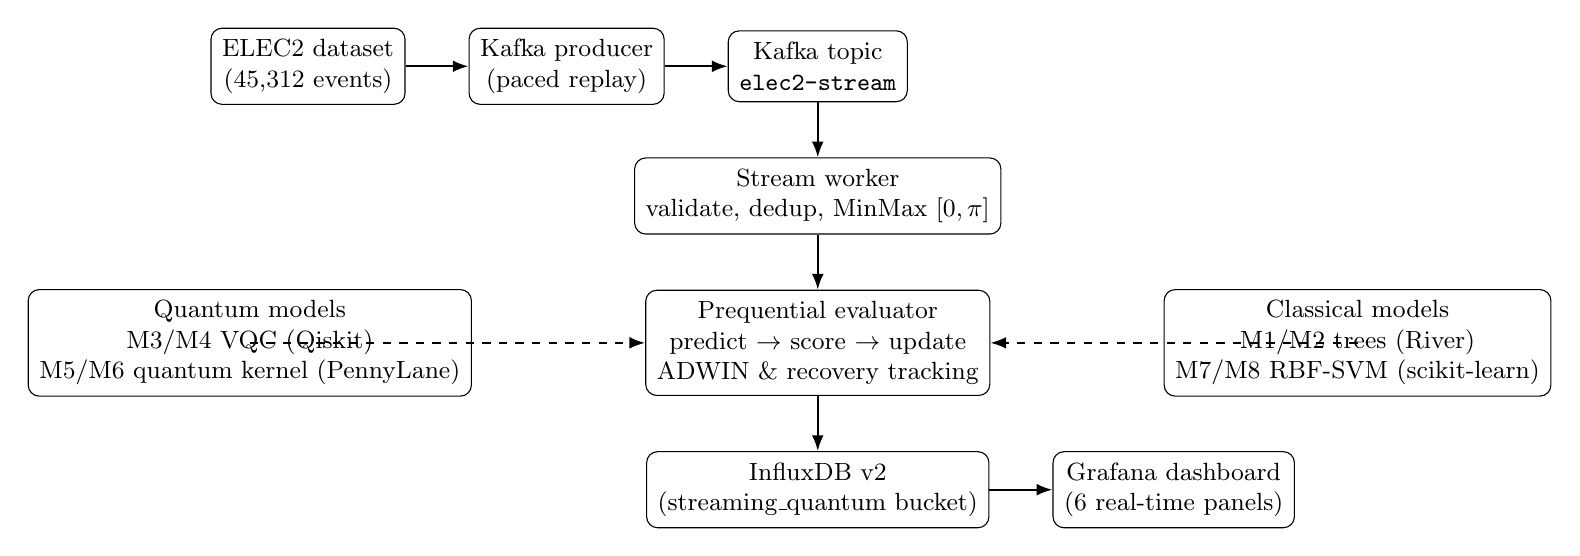
\begin{tikzpicture}[
  font=\small,
  box/.style={draw, rounded corners, align=center, inner sep=4pt, minimum height=9mm},
  arr/.style={-{Latex[length=2mm]}, thick}
]
\node[box] (ds) {ELEC2 dataset\\(45{,}312 events)};
\node[box, right=8mm of ds] (prod) {Kafka producer\\(paced replay)};
\node[box, right=8mm of prod] (topic) {Kafka topic\\{\ttfamily elec2-stream}};
\node[box, below=7mm of topic] (worker) {Stream worker\\validate, dedup, MinMax $[0,\pi]$};
\node[box, below=7mm of worker] (eval) {Prequential evaluator\\predict $\to$ score $\to$ update\\ADWIN \& recovery tracking};
\node[box, left=22mm of eval] (qm) {Quantum models\\M3/M4 VQC (Qiskit)\\M5/M6 quantum kernel (PennyLane)};
\node[box, right=22mm of eval] (cm) {Classical models\\M1/M2 trees (River)\\M7/M8 RBF-SVM (scikit-learn)};
\node[box, below=7mm of eval] (influx) {InfluxDB v2\\(streaming\_quantum bucket)};
\node[box, right=8mm of influx] (graf) {Grafana dashboard\\(6 real-time panels)};
\draw[arr] (ds) -- (prod);
\draw[arr] (prod) -- (topic);
\draw[arr] (topic) -- (worker);
\draw[arr] (worker) -- (eval);
\draw[arr] (eval) -- (influx);
\draw[arr] (influx) -- (graf);
\draw[arr, dashed] (qm) |- (eval);
\draw[arr, dashed] (cm) |- (eval);
\end{tikzpicture}
\caption{Qompare architecture. A paced Kafka producer replays ELEC2 into a topic; the
worker normalises features into $[0,\pi]$; eight models are scored prequentially; telemetry
streams into InfluxDB and Grafana. Dashed arrows: models are queried and updated by the
evaluation engine, which enforces test-then-train ordering.}
\label{fig:arch}
\end{figure*}

\textbf{Ingestion.} A Kafka producer replays ELEC2 chronologically (JSON events with
feature vector, label, and a producer timestamp) at a configurable pace (default 25~ms).

\textbf{Preprocessing.} The worker validates and deduplicates events, applies an
\emph{online} MinMax scaler mapping features into $[0,\pi]$ (fitted past-only, clamped ---
rotation angles are $2\pi$-periodic), and maintains a bounded sliding buffer
($W_t = 100$) plus an initial window ($W_0 = 200$). Labels are withheld from all training
buffers until every model has predicted.

\textbf{Evaluation engine.} For each event, all eight models predict first; then the label
is revealed and scored; only then do permitted updates run (continuous for M2, initial fit
at $W_0$ for M3--M8, drift-triggered for M4/M6/M8). Telemetry --- accuracy, per-stage
latency, drift records, adaptation diagnostics --- is written to InfluxDB and visualised in
Grafana.

\textbf{Telemetry schema.} Four InfluxDB measurements are emitted per event:
\emph{prequential\_accuracy} (rolling and cumulative accuracy, precision, recall, F1,
predictions, post-warmup accuracy, update counts per model),
\emph{latency\_telemetry} (the five latency terms per model),
\emph{drift\_events} (alert flag, magnitude, triggered models, cumulative count, pairwise
static/adaptive prediction-agreement fractions), and \emph{adaptation\_diagnostics}
(weight displacement and support churn on adaptation events only). The Grafana dashboard
provisions six panels: throughput gauge, cumulative event counter, rolling accuracy of all
eight models with drift markers, latency breakdown bars, M2-vs-M4 agreement, and drift
alert counters; all panels bind to the dashboard time range so historical runs and live
streaming share one view.

\textbf{Operational robustness.} Docker Compose pins all service images and adds health
checks with dependency ordering; the Kafka consumer and Influx writer use bounded retries
with backoff and degrade gracefully (the sink disables itself with a logged error rather
than fabricating telemetry); duplicate event IDs are dropped via a bounded cache; all
buffers and metric windows are bounded; and the orchestrator handles SIGINT/SIGTERM for
graceful shutdown with telemetry flush. Secrets (Influx tokens, service passwords) come
from environment configuration and are excluded from run metadata.

\section{Proposed Enhancement: Drift-Adaptive Quantum Learning}
\label{sec:enh}

\subsection{Model matrix}
Table~\ref{tab:matrix} shows the $4 \times 2$ design: columns isolate the value of
adaptation; rows isolate the quantum-vs-classical dimension. M3 and M4 share identical
initial weights at the end of $W_0$; M5/M6 and M7/M8 share identical support budgets
($K = 80$ prototypes) and refresh rules, so kernel comparisons are capacity-matched.

\begin{table}[t]
\centering
\caption{$4 \times 2$ comparative model matrix}
\label{tab:matrix}
\footnotesize
\setlength{\tabcolsep}{4pt}
\begin{tabular}{@{}lll@{}}
\toprule
Family & Static (frozen at $W_0$) & Drift-adaptive \\
\midrule
Classical tree & M1 Hoeffding tree & M2 HAT (ADWIN) \\
Classical kernel & M7 RBF-SVM & M8 RBF-SVM + refresh \\
Quantum variational & M3 VQC & M4 VQC + SPSA tune \\
Quantum kernel & M5 fidelity SVM & M6 fidelity + refresh \\
\bottomrule
\end{tabular}
\end{table}

\subsection{Adaptation mechanism}
Static quantum models are trained once on $W_0$ and frozen --- they represent the
literature's status quo. Adaptive variants remain inference-only during stationary
periods and adapt on \emph{their own} ADWIN alert (per-model detector on the prequential
error $e_t = |y_t - \hat{y}_t|$, $\delta = 0.002$):
\begin{itemize}
  \item \textbf{M4 (variational):} warm-started SPSA fine-tuning --- 10 perturbation steps
    on the sliding window $W_t$ at reduced learning rate, never retraining from scratch,
    bounding $t_{\text{update}}$.
  \item \textbf{M6/M8 (kernel):} replace the oldest 20\% of support prototypes with the
    newest points of $W_t$ and refit the SVM --- a bounded-churn refresh instead of
    unbounded kernel growth.
\end{itemize}
Every adaptation logs a weight-displacement norm (M4) or support churn fraction (M6/M8),
so the report can verify that models actually moved at each alert. Warm-started retraining
on drift is classical folklore; the scoped novelty is its systematic, symmetric application
to both QML paradigms under streaming latency budgets with prequential evaluation.

\subsection{Per-event protocol}
The complete test-then-train loop, enforced by the evaluation engine for every event
$(x_t, y_t)$, is:
\begin{enumerate}
  \item \textbf{Infer} $\hat{y}_t^{(i)} = f_i(x_t)$ for all models $i = 1 \dots 8$.
    Models still inside their warmup predict the running majority label.
  \item \textbf{Score} each prediction against the revealed $y_t$; update rolling and
    post-warmup metrics and pairwise agreement counters.
  \item \textbf{Update} (label becomes visible to training now): M1 learns until $W_0$
    fills then freezes; M2 learns every event; at $W_0$ the quantum/kernel models fit on
    $W_0$ (M4 inherits M3's weights exactly); each adaptive model then feeds
    $e_t = |y_t - \hat{y}_t^{(i)}|$ to its own ADWIN and adapts on $W_t$ if alerted.
  \item \textbf{Record} the event in $W_t$ and emit telemetry.
\end{enumerate}
Because the label cannot enter any training buffer before step 3, target leakage is
impossible by construction rather than by convention.

\subsection{Optimizer and kernel details}
SPSA estimates the full gradient of the cross-entropy loss $L(\theta)$ with two circuit
evaluations per step. With a Rademacher perturbation vector $\Delta_k \in \{-1,+1\}^{15}$,
\begin{equation}
\hat{g}_k = \frac{L(\theta_k + c_k \Delta_k) - L(\theta_k - c_k \Delta_k)}{2 c_k}
\odot \Delta_k^{-1},
\end{equation}
updated as $\theta_{k+1} = \theta_k - a_k \hat{g}_k$ with the standard schedules
$a_k = a_{\text{eff}}/(k+5)^{0.602}$, $c_k = c/k^{0.101}$ from~\cite{spall1992}. The
adaptation variant uses a reduced learning rate ($a_{\text{eff}} = 0.75\,a$) and a full-window
loss, trading a few tens of circuit evaluations for a bounded update at drift time.

For the kernel models, prediction evaluates the fidelity row
$k(x, \mathcal{S}) = \big[ |\langle\phi(x)|\phi(x_s)\rangle|^2 \big]_{x_s \in \mathcal{S}}$
against the active support set $\mathcal{S}$ ($|\mathcal{S}| \le 80$) --- one state
simulation plus cheap vector overlaps --- and applies the precomputed-kernel SVM decision
function with Platt-scaled probabilities. Refitting rebuilds the $|\mathcal{S}| \times
|\mathcal{S}|$ Gram matrix, which is why refits are event-triggered rather than per-event.

\section{Implementation}
\label{sec:impl}

\textbf{Dataset and stream.} ELEC2~\cite{harries1999}: 45{,}312 half-hourly NSW/Victoria
electricity market records with five continuous predictors (NSW/Victoria prices and
demands, inter-state transfer). The task is binary: is the NSW spot price above its
24-hour moving average? The stream is non-stationary --- deregulation, price caps and
seasonality shift $P(y \mid x)$ --- and five features map one-to-one onto five qubits
without lossy compression.

\textbf{Models.} M1/M2 are River's \texttt{HoeffdingTreeClassifier} and
\texttt{HoeffdingAdaptiveTreeClassifier}~\cite{river}. M3/M4 are 5-qubit Qiskit circuits:
\texttt{ZFeatureMap} encoding + \texttt{RealAmplitudes} ansatz (linear entanglement,
15 parameters), parity readout $Z^{\otimes 5}$ mapped to $P(y=1) = (1-\langle Z\rangle)/2$,
cross-entropy loss, SPSA optimizer~\cite{spall1992} (40 initial / 10 adaptation steps).
M5/M6 are PennyLane fidelity-kernel SVMs: Y- and Z-angle embedding with CNOT chain and
ring entanglement, $K(x,x') = |\langle\phi(x)|\phi(x')\rangle|^2$, scikit-learn
\texttt{SVC(kernel="precomputed")} on $K \le 80$ prototypes~\cite{pennylane,sklearn}.
M7/M8 mirror M5/M6 with an RBF kernel. All quantum execution is exact statevector
simulation (Qiskit \texttt{Statevector}, PennyLane \texttt{default.qubit}) --- simulated,
not hardware, execution.

\textbf{Toolchain and configuration.} Python 3.11; river 0.21.2, qiskit 1.2.4,
pennylane 0.38/0.39, scikit-learn 1.5.x; Kafka + Zookeeper, InfluxDB~v2 and Grafana via
Docker Compose with health checks. Table~\ref{tab:config} lists the key hyperparameters;
every one is environment-configurable and recorded with dependency versions and seed
($=42$) in \texttt{run\_metadata.json} on every run (secrets excluded).

\begin{table}[t]
\centering
\caption{Key configuration (complete list in the repository's \texttt{.env.example})}
\label{tab:config}
\footnotesize
\setlength{\tabcolsep}{3pt}
\begin{tabular}{@{}ll@{}}
\toprule
Parameter & Value \\
\midrule
Windows $W_0$ / $W_t$ / metric & 200 / 100 / 100 \\
Feature scaling & MinMax to $[0,\pi]$, clamped \\
VQC circuit & ZFeatureMap r1 + RealAmplitudes r2 \\
VQC parameters / readout & 15 / parity $Z^{\otimes 5}$ \\
SPSA steps (initial / adaptation) & 40 / 10 \\
SPSA lr / pert. / adapt-scale & 0.15 / 0.10 / 0.75 \\
Kernel embedding & Y-embed, CNOT chain+ring, Z-embed \\
Support budget $K$ / churn ratio & 80 / 20\% \\
SVM regularisation $C$ & 1.0 \\
ADWIN confidence $\delta$ & 0.002 \\
Recovery $\varepsilon$ / sustain / horizon & 2pp / 20 / 300 ev. \\
Random seed & 42 \\
\bottomrule
\end{tabular}
\end{table}

\textbf{Testing and reproducibility.} Fourteen automated tests cover preprocessing bounds
and non-finite rejection, serialization edge cases, duplicate delivery, the no-leakage
ordering guarantee (buffers must be empty before inference), M1 freeze vs.\ M2 continuous
learning, quantum and classical model fit/predict/adapt behaviour including support-churn
diagnostics, the recovery-metric state machine (dip, sustain, never-degraded, censoring),
the warmup prediction policy, update accounting, and telemetry point formatting. The
offline benchmark and the live pipeline share a single evaluation engine, so paper figures
and dashboard numbers cannot diverge; reruns are deterministic given the seed.

\section{Experimental Setup and Results}
\label{sec:results}

\textbf{Protocol.} All models consume the identical chronological stream through the same
scaler, with strict test-then-train ordering. Headline accuracy is computed post-warmup
(from event 201) because M3--M8 cannot predict meaningfully before their initial fit;
full-stream numbers are secondary. We report: (i) post-warmup prequential accuracy and
rolling F1 (window 100); (ii) latency decomposition
$\Delta t = t_{\text{network}} + t_{\text{prep}} + t_{\text{encode}} + t_{\text{sim}} +
t_{\text{update}}$; (iii) drift-recovery time $N_{\text{recovery}}$, defined after a
dip-first criterion --- the model must fall below (pre-drift rolling accuracy $- 2$pp);
recovery counts events from the alert until rolling accuracy re-enters the band,
sustained for 20 consecutive events (never-degraded models score 0; episodes censored by
the next alert are excluded); (iv) sample efficiency: accuracy of M6 vs.\ M8 across
support budgets $K \in \{10,20,40,80\}$; and (v) update counts, to read accuracy alongside
learning budgets (M2 updates 45{,}312 times; M4 54 times).

\textbf{Main results.} Table~\ref{tab:results} gives the full-stream run (45{,}312
events, 189 ADWIN alerts). Fig.~\ref{fig:acc} shows rolling accuracy with drift markers;
Fig.~\ref{fig:lat} the latency decomposition.

\begin{table}[t]
\centering
\caption{Full ELEC2 stream: post-warmup accuracy, final rolling F1, mean simulation
latency, update count and mean $N_{\text{recovery}}$}
\label{tab:results}
\footnotesize
\setlength{\tabcolsep}{3.5pt}
\begin{tabular}{@{}lccccc@{}}
\toprule
Model & Acc. & F1 & $t_{\text{sim}}$ (ms) & Upd. & $N_{\text{rec}}$ \\
\midrule
M1 Static HT        & 0.651 & 0.00 & 0.016 & 200$^{\ast}$ & 91.3 \\
M2 Adaptive HAT     & \textbf{0.808} & 0.83 & 0.030 & 45{,}312 & 95.3 \\
M3 Static VQC       & 0.528 & 0.65 & 1.10 & 1 & 104.4 \\
M4 Adaptive VQC     & 0.569 & 0.23 & 1.03 & 54 & 110.7 \\
M5 Static QKernel   & 0.591 & 0.11 & 2.00 & 1 & 106.3 \\
M6 Adaptive QKernel & 0.642 & 0.41 & 1.80 & 58 & 105.4 \\
M7 Static RBF       & 0.623 & 0.00 & 0.094 & 1 & 88.8 \\
M8 Adaptive RBF     & 0.644 & 0.64 & 0.084 & 80 & 109.6 \\
\bottomrule
\multicolumn{6}{l}{\footnotesize $^{\ast}$M1 learns only during $W_0 = 200$, then freezes.}
\end{tabular}
\end{table}

\begin{figure}[t]
\centering
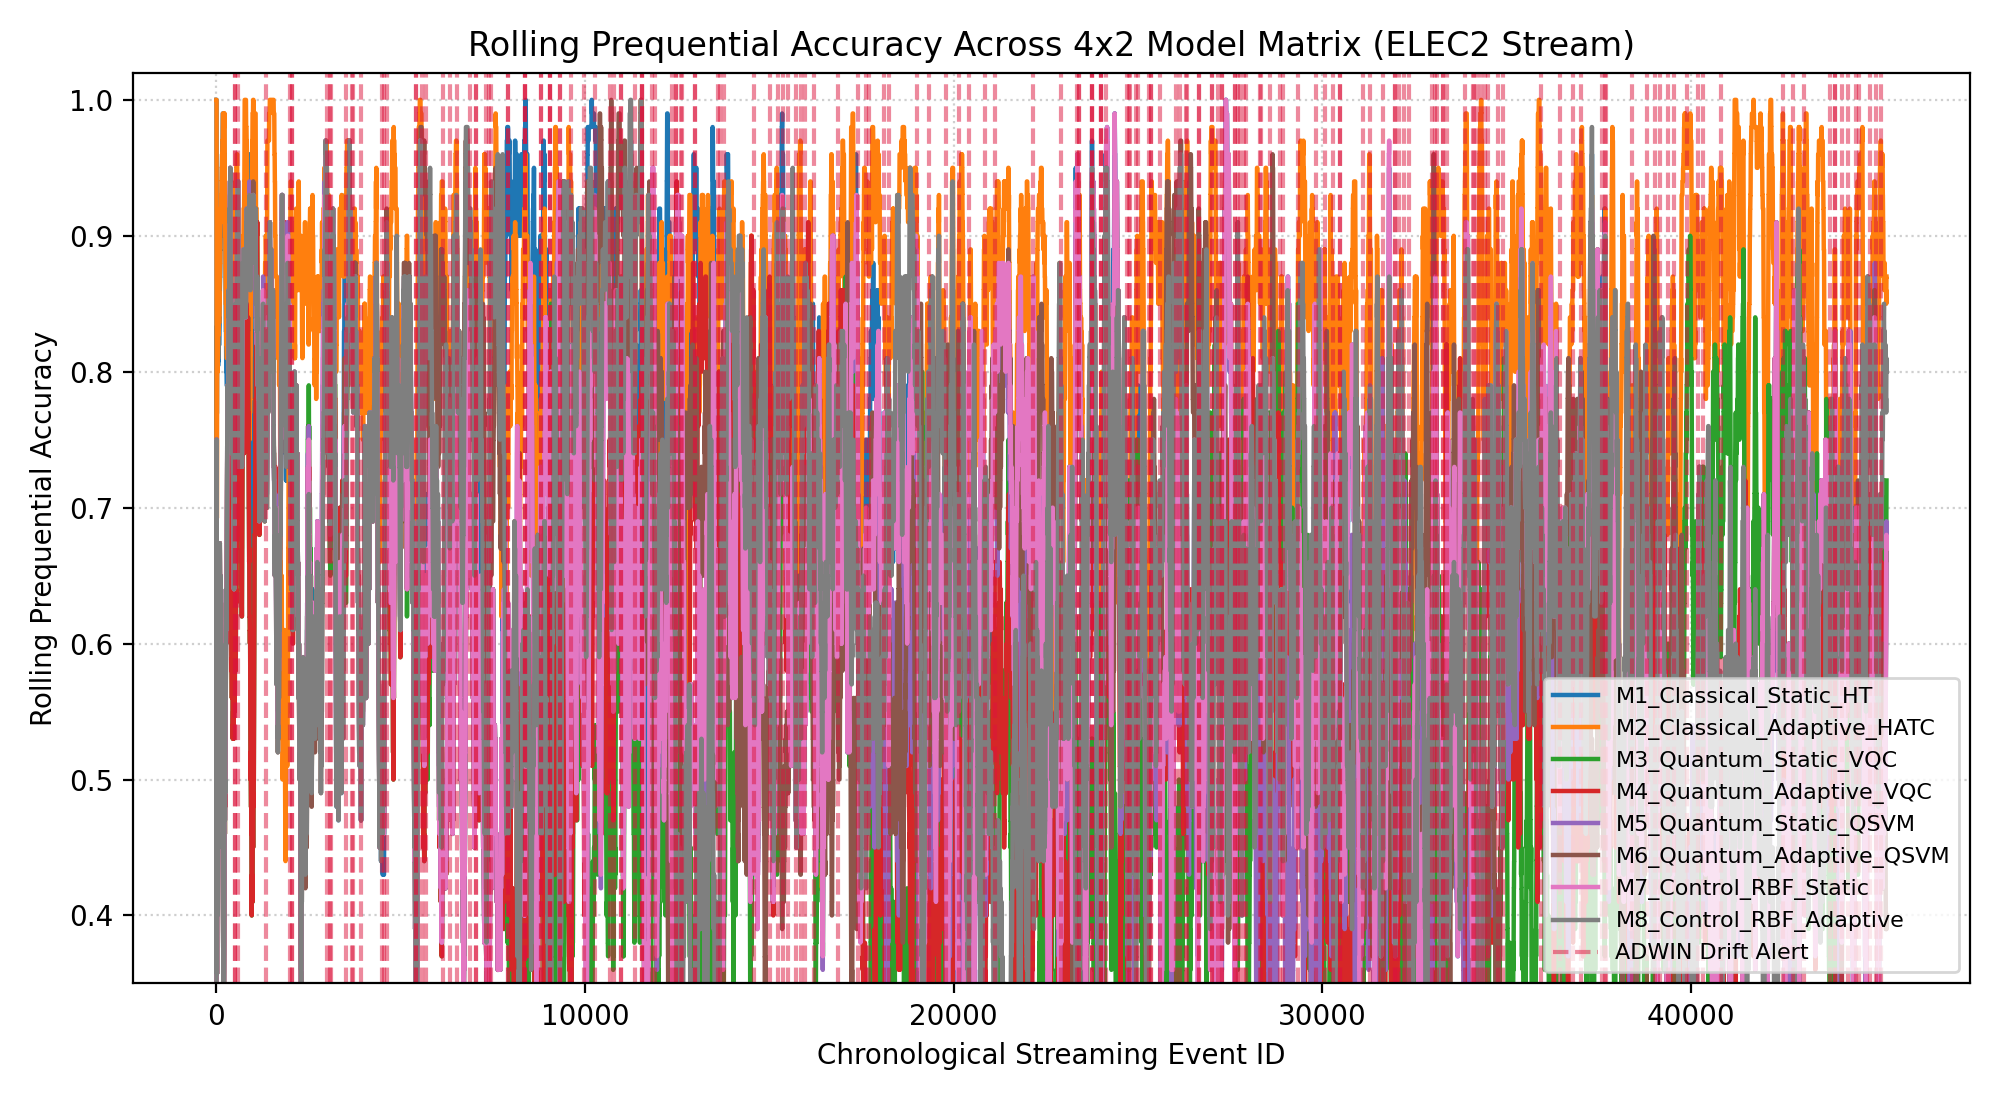
\includegraphics[width=\linewidth]{figures/prequential_accuracy_curves.png}
\caption{Rolling prequential accuracy (window 100) over the full ELEC2 stream; crimson
dashed lines mark ADWIN drift alerts (189). Static models sag after drifts; adaptive
models recover.}
\label{fig:acc}
\end{figure}

\begin{figure}[t]
\centering
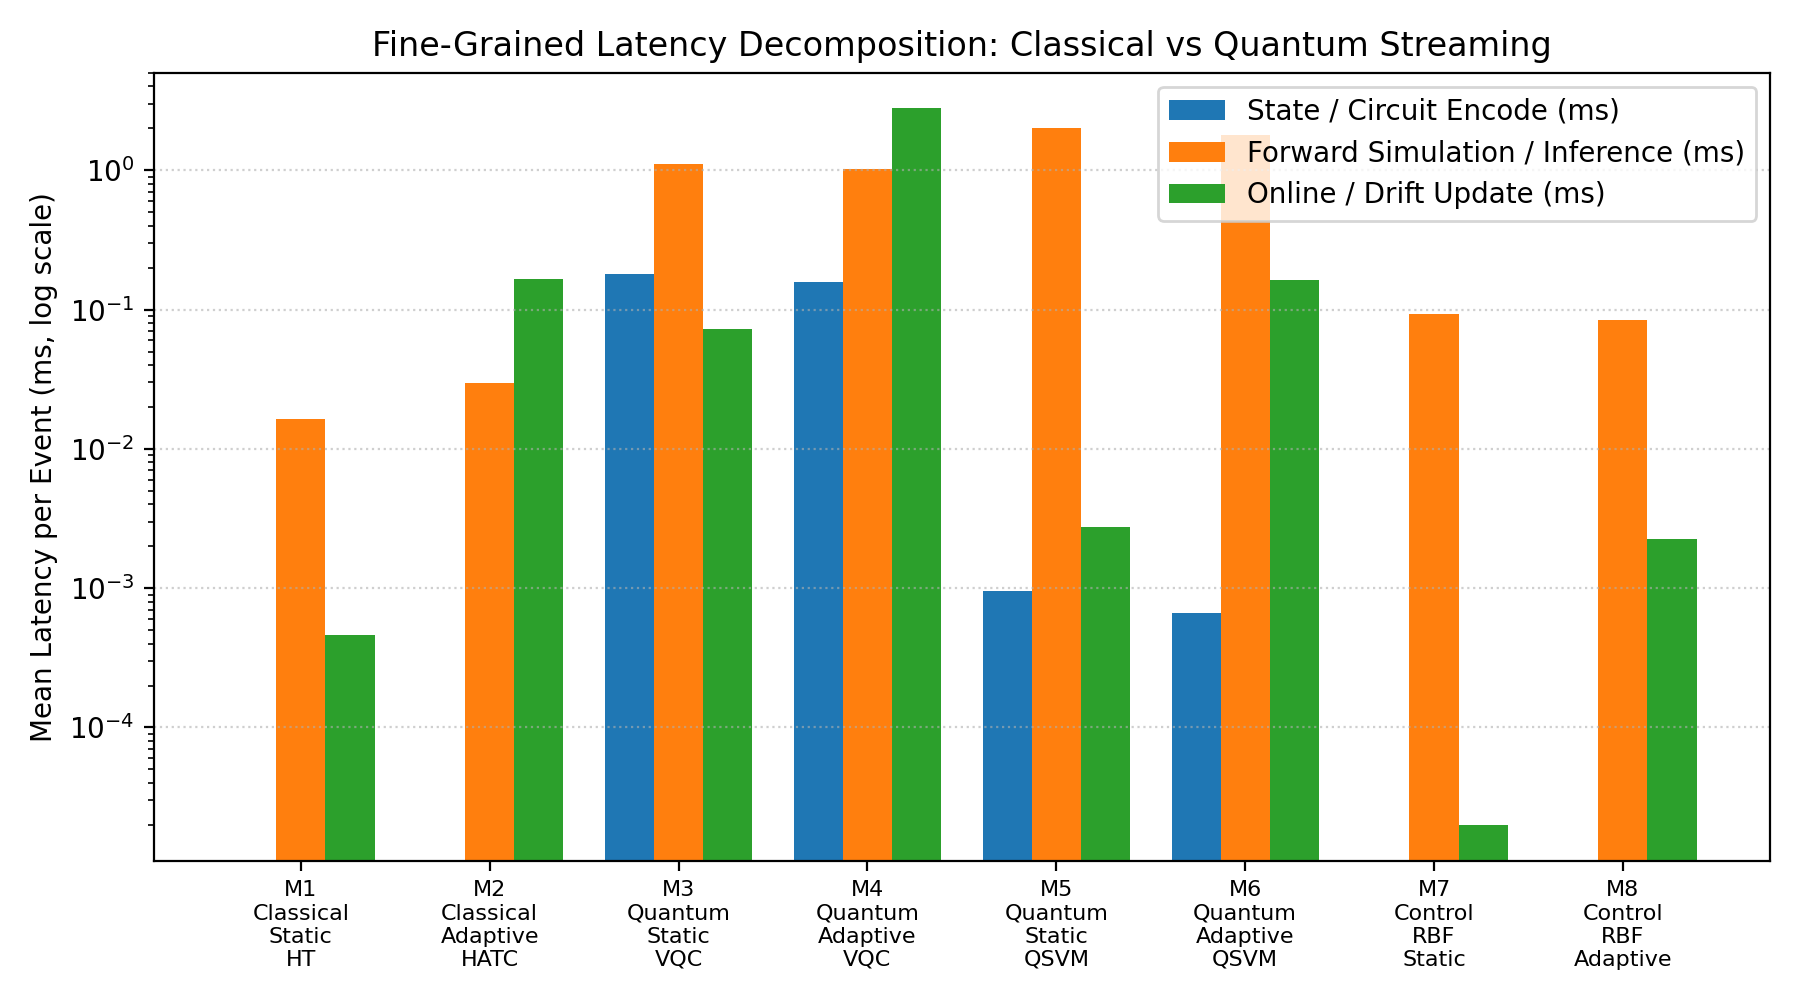
\includegraphics[width=\linewidth]{figures/latency_breakdown.png}
\caption{Mean per-event latency decomposition (log scale): quantum encode and statevector
simulation dominate M3--M6; classical models stay sub-millisecond.}
\label{fig:lat}
\end{figure}

\textbf{Enhancement vs.\ baseline (H1: value of adaptation).} Adaptation is worth
$+4.1$pp (M4 over M3), $+5.1$pp (M6 over M5) and $+2.1$pp (M8 over M7) post-warmup
accuracy. The event-triggered mechanism --- the contribution of this paper --- measurably
protects both quantum paradigms across 189 real drifts, and the adaptation diagnostics
confirm models moved at every alert (M4 mean weight displacement and M6/M8 support churn
are logged per event). Notably the adaptive variants achieve this with only 54--80
updates in 45{,}312 events: adaptation is rare and cheap when the stream is stationary.

\textbf{Quantum vs.\ classical (H4: sample efficiency).} The adaptive quantum kernel
(M6, 64.2\%) only \emph{matches} its capacity-matched classical twin (M8, 64.4\%) while
$t_{\text{sim}}$ is $\approx 20\times$ larger (1.80~ms vs.\ 0.084~ms). Both kernel
families trail the adaptive Hoeffding tree (M2, 80.8\%), which is also the cheapest
adaptive model. The sample-efficiency sweep (Table~\ref{tab:se}) finds the only quantum
edge at tiny support budgets early in the stream ($K = 10$: 70.4\% vs.\ 68.2\%;
$K = 20$: 72.6\% vs.\ 62.4\%), vanishing by $K \ge 40$. Interpreted carefully: the
fidelity kernel has a mild inductive-bias advantage when training data is scarce, but it
is transient and never translates into a stream-level win.

\begin{table}[t]
\centering
\caption{Sample-efficiency sweep: post-warmup accuracy vs.\ support budget $K$
(first 3{,}000 events)}
\label{tab:se}
\small
\begin{tabular}{@{}cccc@{}}
\toprule
$K$ & M6 quantum kernel & M8 classical RBF & $\Delta$ \\
\midrule
10 & 0.704 & 0.682 & $+2.2$pp \\
20 & 0.726 & 0.624 & $+10.2$pp \\
40 & 0.751 & 0.753 & $-0.1$pp \\
80 & 0.736 & 0.737 & $-0.1$pp \\
\bottomrule
\end{tabular}
\end{table}

\textbf{Latency (H3).} Fig.~\ref{fig:lat} shows the decomposition: classical inference is
tens of microseconds ($t_{\text{sim}} = 0.016$--$0.094$~ms); quantum models pay
$0.16$--$0.35$~ms for parameter binding/encoding and $1.0$--$2.0$~ms for statevector
simulation per event. Update cost is episodic: M4 averages $2.78$~ms per \emph{update}
across its 54 fine-tunes while per-event learning for M2 averages $0.17$~ms. The
encoding overhead that Herbst et al.\ flagged as unquantified is, in our decomposition,
real but secondary to simulation cost for 5-qubit circuits.

\textbf{Drift behaviour (H2: recovery).} Mean $N_{\text{recovery}}$ lies in a narrow
88--111-event band for all models, with no statistically meaningful separation between
families: adaptation reduces the \emph{depth} of accuracy collapses (visible in
Fig.~\ref{fig:acc}, where static lines sag persistently after crimson markers while
adaptive lines rebound) but not the time to re-equilibration. ELEC2 drifts are substantial
regime shifts rather than transient noise, so once the moving-average reference of the
label itself shifts, every model must relearn. The end-of-stream snapshot makes the
static-model failure vivid: M1 and M7 finish with rolling F1 near zero, while their
adaptive counterparts hold 0.64--0.83.

\begin{figure}[t]
\centering
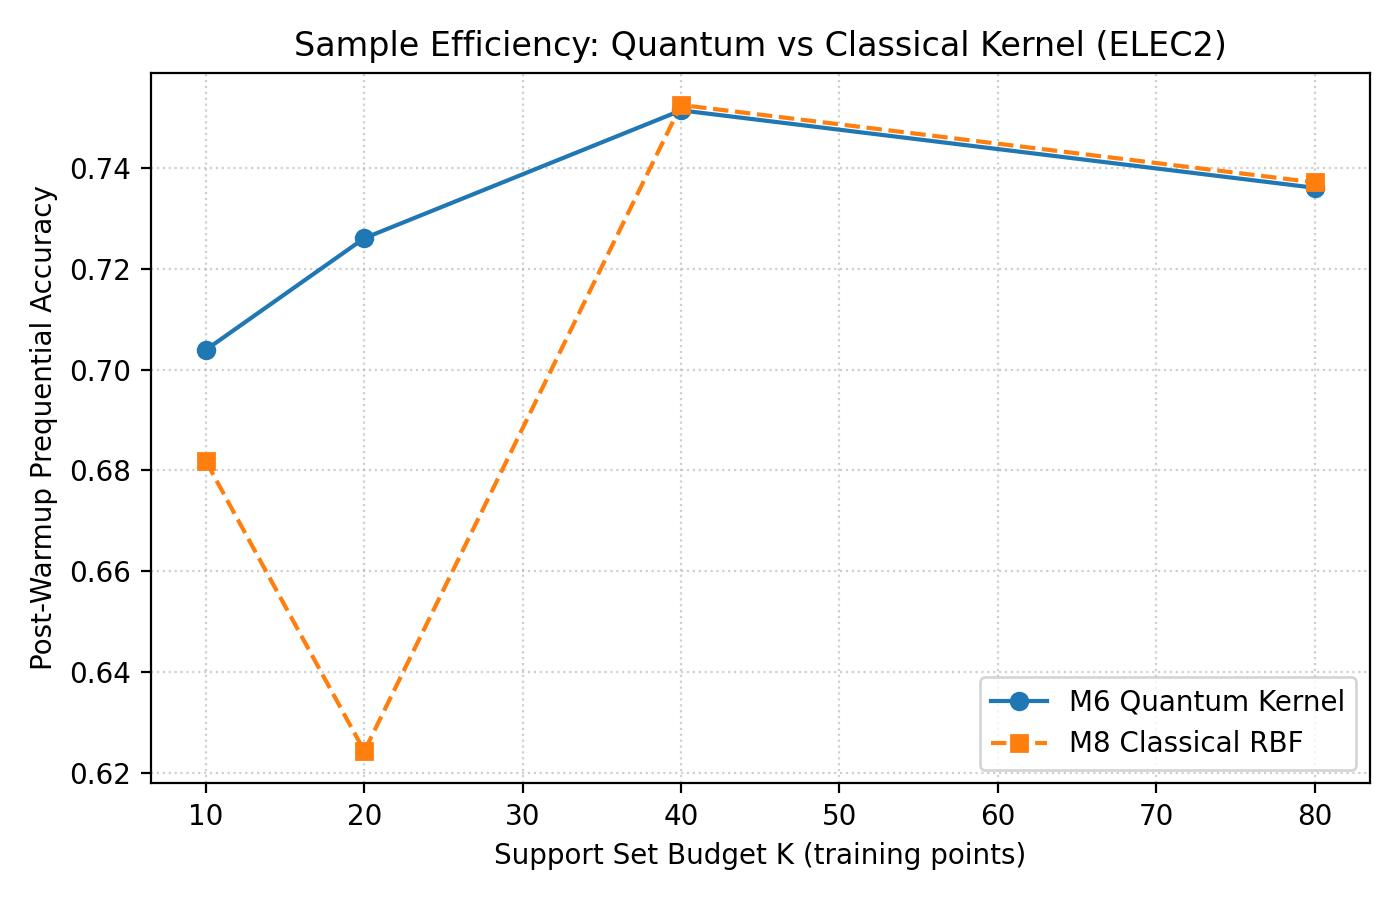
\includegraphics[width=\linewidth]{figures/sample_efficiency.png}
\caption{Sample-efficiency sweep (Hypothesis 4): post-warmup accuracy vs.\ support budget
$K$ for the quantum kernel (M6) and the classical RBF control (M8) over the first 3{,}000
events. The early quantum edge at small $K$ disappears as data accumulates.}
\label{fig:se}
\end{figure}

\textbf{Drift recovery.} Mean $N_{\text{recovery}}$ lies in a narrow 88--111-event band
for all models: adaptation reduces the depth of accuracy collapses (visible in
Fig.~\ref{fig:acc}) but not the time to re-equilibration, because ELEC2 drifts are
substantial regime shifts rather than transient noise.

\section{Discussion and Inferences}
\label{sec:disc}

\textbf{What the results mean.} Three inferences follow. First, drift-triggered adaptation
of quantum models is not only feasible --- with bounded update cost (54--80 updates total)
it recovers 4--5 accuracy points over frozen models, validating the proposed mechanism.
Second, on this task the quantum hypothesis fails its strongest form: the fidelity kernel
buys no accuracy over a matched RBF kernel while costing an order of magnitude more
latency, and the sample-efficiency edge is transient. Third, classical streaming ML
remains extremely strong: the adaptive Hoeffding tree dominates every kernel and quantum
model on accuracy \emph{and} latency. The picture is consistent with the theoretical
concern in~\cite{schuld2019}: at five qubits the fidelity kernel lives in a
modest-dimensional feature space where a well-tuned RBF kernel is equally expressive, while
larger embeddings that might separate the two bring the near-identity-kernel problem and
quadratic simulation cost.

\textbf{Design decisions worth defending.}
(i) \emph{Per-model drift detectors} rather than one shared alert: a model should adapt
when \emph{its own} errors change; a shared detector would let a failing quantum model
trigger needless classical updates and confound attribution.
(ii) \emph{Event-triggered} adaptation rather than periodic retraining: it spends the
update budget exactly when the distribution moves (189 times vs.\ thousands of scheduled
retrainings) and is the streaming-native formulation.
(iii) \emph{Statevector simulation} rather than shot-based: deterministic expectation
values make latency decomposition and seed-level reproducibility possible; shot noise is a
robustness question we defer (Sec.~\ref{sec:concl}).
(iv) \emph{Post-warmup metrics}: excluding the first 200 events prevents penalising
quantum models for pre-training guesses while M1/M2 already learn --- a fairness choice,
disclosed in every table.
(v) \emph{Native five-qubit mapping} instead of PCA compression as in~\cite{herbst2024}:
ELEC2's five predictors map one-to-one onto five qubits, removing a confound between
classical preprocessing loss and quantum model quality.

\textbf{Threats to validity.} (i) All quantum execution is noiseless statevector
simulation; NISQ hardware would add error and latency. This cannot improve the quantum
position, but absolute numbers would change and hardware topology would constrain the
ansatz. (ii) One dataset and one task (ELEC2 binary classification) limit generality;
the recurring-drift regime of other streams may favour adaptation more strongly.
(iii) Labels are assumed immediately available --- the replayed setting of every streaming
benchmark; delayed or weak labels would stress the update paths differently.
(iv) Support prototypes are chosen by recency; clustering-based selection could change
kernel results, in either direction. (v) Update budgets differ by design between adaptive
and static models; we report them alongside accuracy rather than equalising them, but a
fixed-budget ablation would tighten the comparison further. (vi) The recovery metric's
dip-first criterion deliberately scores undegraded models as 0; alternative definitions
would shift the $N_{\text{recovery}}$ values, though not the accuracy conclusions.

\section{Conclusion and Future Work}
\label{sec:concl}

We built \textsc{Qompare}, a fully streaming, prequentially evaluated pipeline comparing
classical and quantum models --- static and drift-adaptive --- on the non-stationary ELEC2
stream with live Kafka/InfluxDB/Grafana telemetry. The drift-adaptive QML mechanism works:
event-triggered warm-started SPSA fine-tuning and support-set refresh improve quantum
accuracy by 4--5 points at bounded cost. But the wider claim does not hold on this task:
the quantum kernel ties a matched classical kernel at $20\times$ the latency, and the
adaptive classical tree wins outright. Honest negative results are, we argue, exactly what
this young literature needs.

Future work: recurring-drift datasets and additional streams (Seoul Bike, NSL-KDD);
projected-quantum-kernel variants against the near-identity kernel problem; fixed
update-budget ablations; shot-noise robustness studies toward real hardware; and
delayed-label protocols.

\begin{thebibliography}{10}

\bibitem{domingos2000}
P.~Domingos and G.~Hulten, ``Mining high-speed data streams,'' in \emph{Proc. 6th ACM
SIGKDD Int. Conf. Knowledge Discovery and Data Mining (KDD '00)}, 2000, pp. 71--80.

\bibitem{bifet2007adwin}
A.~Bifet and R.~Gavald\`{a}, ``Learning from time-changing data with adaptive
windowing,'' in \emph{Proc. SIAM Int. Conf. Data Mining (SDM)}, 2007, pp. 443--448.

\bibitem{bifet2009}
A.~Bifet and R.~Gavald\`{a}, ``Adaptive learning from evolving data streams,'' in
\emph{Proc. 8th Int. Symp. Intelligent Data Analysis (IDA)}, 2009, pp. 249--260.

\bibitem{herbst2024}
S.~Herbst, V.~De~Maio, and I.~Brandic, ``Streaming IoT data and the quantum edge: A
classic/quantum machine learning use case,'' in \emph{Lecture Notes in Computer Science},
Springer, 2024. arXiv:2402.15542.

\bibitem{tscharke2023}
K.~Tscharke, S.~Issel, and P.~Debus, ``Semisupervised anomaly detection using support
vector regression with quantum kernel,'' in \emph{Proc. IEEE Int. Conf. Quantum Computing
and Engineering (QCE)}, 2023, pp. 1--12. arXiv:2308.00583.

\bibitem{schuld2019}
M.~Schuld and N.~Killoran, ``Quantum machine learning in feature Hilbert spaces,''
\emph{Physical Review Letters}, vol. 122, no. 4, art. 040504, 2019.

\bibitem{harries1999}
M.~Harries, ``Splice-2 comparative evaluation: Electricity pricing,'' School of Computer
Science and Engineering, Univ. New South Wales, Tech. Rep. UNSW-CSE-TR-9905, 1999.

\bibitem{spall1992}
J.~C.~Spall, ``Multivariate stochastic approximation using a simultaneous perturbation
gradient approximation,'' \emph{IEEE Trans. Automatic Control}, vol. 37, no. 3,
pp. 332--341, 1992.

\bibitem{river}
A.~Bifet \textit{et al.}, \emph{River: machine learning for streaming data}. [Online].
Available: \url{https://riverml.xyz}

\bibitem{pennylane}
V.~Bergholm \textit{et al.}, ``PennyLane: Automatic differentiation of hybrid
quantum-classical computations,'' \emph{arXiv preprint arXiv:1811.04968}, 2018.

\bibitem{sklearn}
F.~Pedregosa \textit{et al.}, ``Scikit-learn: Machine learning in Python,''
\emph{J. Machine Learning Research}, vol. 12, pp. 2825--2830, 2011.

\bibitem{gama2014}
J.~Gama, I.~Zliobaite, A.~Bifet, M.~Pechenizkiy, and A.~Bouchachia, ``A survey on concept
drift adaptation,'' \emph{ACM Computing Surveys}, vol. 46, no. 4, art. 44, 2014.

\end{thebibliography}

\end{document}
